\documentclass[8pt]{beamer}
\usetheme{CambridgeUS}
\usepackage{pgfpages}
\usepackage{graphicx}
\usepackage{amsfonts}
\usepackage{times}
%\usepackage[usenames]{color}
%\usepackage{color}
\usepackage{tcolorbox}
\usepackage{wrapfig}

\def\'#1{\if#1i{\accent 19\i}\else{\accent 19 #1}\fi}
\def\mb#1{\mbox{\boldmath $#1$}}
\def\ts#1{{\textstyle #1}}
\def\ss#1{{\scriptscriptstyle #1}}
\def\ssr#1{{\scriptscriptstyle\rm #1}}
\def\onehalf{{\textstyle\frac12}}
\def\ds#1{{\displaystyle #1}}
\def\ket#1{| #1 \rangle}
\def\bra#1{{\langle #1 |}}
\def\onesqrt2{{\textstyle \frac{1}{\sqrt{2}}}}
\def\onequarter{{\textstyle \frac14}}	
\def\oneoct{{\textstyle \frac18}}	
\def\onenfac{{\textstyle \frac1{\sqrt{n!}}}}
\def\EExp{{\large e}}
\def\veec{\mathbin{\put(-3,2.6){\line(1,0){50}} \hspace{1.3cm} \succ}}
\def\veecshort{\mathbin{\put(-3,2.6){\line(1,0){30}} \hspace{0.7cm} \succ}}
\def\veeco{\mathbin{\put(-5,2.6){\line(1,0){50}} \hspace{1.2cm} \rightarrow}}
\def\underlim#1{\smash{\mathop{\veec}\limits_{#1}}}
\def\overlim#1{\smash{\mathop{\veec}\limits^{#1}}}
\def\underlimshort#1{\smash{\mathop{\veecshort}\limits_{#1}}}
\def\onehalf{{\textstyle \frac12}}
\def\onesqrt{{\textstyle \frac{1}{\sqrt{2}}}}
\def\onequarter{{\textstyle \frac14}}	
\def\oneoct{{\textstyle \frac18}}	
\def\onenfac{{\textstyle \frac1{\sqrt{n!}}}}
\def\EExp{{\LARGE{e}}}
\def\vecdos#1#2{{ \begin{pmatrix}  #1  \\ #2 \end{pmatrix}}}
\def\vectres#1#2#3{{\left(\begin{matrix}  #1\vspace{-4pt} \\ \vspace{-6pt} #2  \\ #3 \vspace{3pt} \end{matrix}\right)}}
\def\matdos#1#2#3#4{{ \small{ \Bigg( \begin{matrix}  \vspace{6pt} 
#1\hspace{-4pt} &\vspace{-7pt} #2 \\ \vspace{0pt}
#3\hspace{-4pt} &\vspace{2pt} #4
\end{matrix}\hspace{1pt}} \Bigg) }}	
									% para origen palabra
\def\matdosi#1#2#3#4{{ \bigg( \small{ \begin{matrix}  \vspace{6pt} 
#1\hspace{-5pt} &\vspace{-11pt} #2 \\ \vspace{0pt}
#3\hspace{-5pt} &\vspace{2pt} #4
\end{matrix}\hspace{1pt}} \bigg)^{-1} }}		
\def\mattres#1#2#3#4#5#6#7#8#9{{ \left( \begin{matrix}  \vspace{6pt} 
#1\hspace{-5pt} & #2 &\vspace{-11pt} #3 \\ \vspace{-4pt}
#4 & #5 & #6 \\ \vspace{0pt}
#7\hspace{-5pt} & #8 & \vspace{2pt} #9
\end{matrix}\hspace{1pt} \right) }}							
\def\bin#1#2{{\bigg( \hspace{-3pt} \begin{array}{c} \vspace{-4pt}
#1 \vspace{-2pt} \\ \vspace{2pt}  #2
\end{array}  \hspace{-3pt} \bigg) }}
\def\ssr#1{{\scriptscriptstyle\rm #1}}
\def\tsty#1#2{{\textstyle\frac{#1}{#2}}}
\def\ii{{\text{i}}}
\def\dd{{\text{d}}}
\def\sp{{\textsf{sp}}}
\def\Sp{{\textsf{Sp}}}
\def\SU{{\textsf{SU}}}
\def\SO{{\textsf{SO}}}
\def\su{{\textsf{su}}}
\def\u{{\textsf{u}}}
\def\U{{\textsf{U}}}
\def\SLR2{{\textsf{SL}(2,\mathbb{R})}}
\def\SL2C{{\textsf{SL}(2,\mathbb{C})}}
\def\soplus{{\leftarrow \hspace{-11.5pt} \oplus}}
\def\sotimes{{\leftarrow \hspace{-11.5pt} \otimes}}
\def\oG{{\mathcal{G}}}
\newcommand{\eff}{\mathrm{eff}}
\newcommand{\sub}[1]{_{#1}}
\definecolor{ashgrey}{rgb}{0.7, 0.75, 0.71} 
\definecolor{lightgray}{rgb}{0.83, 0.83, 0.83}
\definecolor{flame}{rgb}{0.89, 0.35, 0.13}
\definecolor{persimmon}{rgb}{0.93, 0.35, 0.0}
\definecolor{persianred}{rgb}{0.8, 0.2, 0.2}
\definecolor{cadetblue}{rgb}{0.37, 0.62, 0.63}
\definecolor{cadetgrey}{rgb}{0.57, 0.64, 0.69}
\definecolor{ceil}{rgb}{0.57, 0.63, 0.81}
\definecolor{amber}{rgb}{1.0, 0.49, 0.0}
\definecolor{airforceblue}{rgb}{0.36, 0.54, 0.66}
\definecolor{aqua}{rgb}{0.0, 1.0, 1.0}
\definecolor{brickred}{rgb}{0.8, 0.25, 0.33}
\definecolor{brightlavender}{rgb}{0.75, 0.58, 0.89}
\definecolor{cadetgrey}{rgb}{0.57, 0.64, 0.69}
\definecolor{chocolate}{rgb}{0.48, 0.25, 0.0}
\definecolor{columbiablue}{rgb}{0.61, 0.87, 1.0}
\definecolor{coralpink}{rgb}{0.97, 0.51, 0.47}
\definecolor{darkolivegreen}{rgb}{0.33, 0.42, 0.18}
\definecolor{olive}{rgb}{0.5, 0.5, 0.0}
%\newcommand{\eff}{\mathrm{eff}}
\newcommand{\unit}{{}_{\mathrm{U}} }
\renewcommand{\>}{\rangle}
\newcommand{\<}{\langle}
\newtcolorbox{mybox}[1]
{colback=gray!5!white,colframe=gray!75!black,fonttitle=\bfseries,title=#1}
\newtcolorbox{mygreenbox}[1]
{colback=green!5!white,colframe=green!50!black,fonttitle=\bfseries,title=#1}
\newtcolorbox{myredbox}[1]
{colback=red!5!white,colframe=red!75!white,fonttitle=\bfseries,title=#1}
\newtcolorbox{mybluebox}[1]
{colback=blue!5!white,colframe=blue!75!white,fonttitle=\bfseries,title=#1}
\newcommand{\rmt}{\mathrm{t}}
%----------------------------------------------------------------
\setbeamercolor*{structure}{bg=airforceblue!20,fg=airforceblue}

\setbeamercolor*{palette primary}{use=structure,fg=white,bg=structure.fg}
\setbeamercolor*{palette secondary}{use=structure,fg=white,bg=structure.fg!50!white}
\setbeamercolor*{palette tertiary}{use=structure,fg=white,bg=structure.fg!100!airforceblue}
\setbeamercolor*{palette quaternary}{fg=white,bg=black}

\setbeamercolor{section in toc}{fg=black,bg=airforceblue}
\setbeamercolor{alerted text}{use=structure,fg=structure.fg!50!black!80!black}

\setbeamercolor{titlelike}{parent=palette primary,fg=structure.fg!50!black}
\setbeamercolor{frametitle}{bg=gray!10!white,fg=black}

\setbeamercolor*{titlelike}{parent=palette primary}
%----------------------------------------------------------------


\mode<presentation>
{

 %\usefonttheme{sansserif}
 \setbeamercovered{transparent}
} 

\newcommand{\be}{\begin{equation}}
\newcommand{\ee}{\end{equation}}
\newcommand{\bea}{\begin{eqnarray}}
\newcommand{\eea}{\end{eqnarray}}
\newcommand{\rd}{\bigtriangledown}
\newcommand{\ru}{\bigtriangleup}
\def\matdos#1#2#3#4{{ \small{ \Bigg( \begin{matrix}  \vspace{6pt} 
#1\hspace{-4pt} &\vspace{-7pt} #2 \\ \vspace{0pt}
#3\hspace{-4pt} &\vspace{2pt} #4
\end{matrix}\hspace{1pt}} \Bigg) }}	
\setbeamercolor{postit}{fg=black,bg=cadetblue}
%\sffamily

\title[Teorema KAM] % (optional, use only with long paper titles)
{\huge {Teorema KAM}}

%\subtitle[Física Cuántica y Fotónica]
%{\normalsize{Seminario del Departamento de Física Cuántica y Fotónica}} % (optional)

%\author[Kenan Uriostegui] % (optional, use only with lots of authors)
%{\normalsize{Roberto Kenan Uriostegui Uma\~na}\\[0pt]
% \texttt{\small rkenanuu@fisica.unam.mx}}
%  
%\institute[IFUNAM]{}
%  \inst{}%
%  \normalsize{{\bf Instituto de F\'isica\\
%  Universidad Nacional Aut\'onoma de M\'exico}}}

%\date[1/3/2023] % (optional)
%{\scriptsize 1 de marzo, 2023}

\begin{document}
%\pgfdeclareimage[height=2cm]{institute-logo}{logoIF.jpg}
%\logo{\pgfuseimage{institute-logo}}
%-----------------------------------------------
\begin{frame}[plain,noframenumbering]
%\vspace{0.6cm}
%\hspace{0.2cm}\includegraphics[height=2cm]{escudo_unam.jpg}
%\hfill
%\includegraphics[height=2cm]{logoIF.jpg}
\titlepage 

%\begin{center}
%\centering
%\begin{beamercolorbox}[sep=1em,wd=4cm,ht=1cm,rounded=true,shadow=true,center]{postit}
%\normalsize{Seminario\\ Física Cuántica y Fotónica}
%\end{beamercolorbox}
%\end{center}

\end{frame}
%----------------------------------------------
%\usebackgroundtemplate{\parbox[b][\paperheight][b]{\paperwidth}{\centering\includegraphics[height=\paperheight]{logoUNAM2.png}}}
%
%\setbeamercolor{background canvas}{bg=gray}
%
%\begin{frame}[plain,noframenumbering]
%  \titlepage 
%  \vspace{-2cm} 
%\includegraphics[height=2cm]{logoUNAM3.png}
%\hfill
%\includegraphics[height=1.8cm]{logoIF.jpg}
%\end{frame}


\section[Introducción]{Introducción}

\subsection[Historia]{Historia}

\begin{frame}
{\structure{\Large Algo de historia}}
\vspace{-5cm}

\begin{itemize}
\pause
\item[1954] $\longrightarrow$ Andre\"i Nikolaevich Kolmogorov enuncia El Teorema en el International Congress of \\ \hspace{13pt} Mathematicians en Amsterdam. \pause
\item[1957] $\longrightarrow$ Kolmogorov lo vuelve a discutir en otra edición del mismo congreso.
\pause
\item[1961] $\longrightarrow$ Vladimir Arnold usa las ``técnicas de prueba'' de Kolmogorov para resolver el mapeo \\ \hspace{13pt} circular que antes no había podido ser tratado.
\pause
\item[1962] $\longrightarrow$ J\"urgen Moser combina las ``técnicas de prueba'' de Kolmogorov con otros métodos para \\ \hspace{13pt} probar una versión de baja dimensionalidad del Teorema de Kolmogorov usando una \\ \hspace{13pt} hipótesis débil.
\pause
\item[1963] $\longrightarrow$ Arnold prueba una versión del Teorema de Kolmogorov válida en todas dimensiones.
\pause
\item[1968] $\longrightarrow$ F.M. Izrailev y B.V. Chirikov acuñan el término KAM para la teoría desarrollada en torno \\ \hspace{13pt} a este Teorema (también llamado teorema KAM en la actualidad). 
\end{itemize}
\pause
\begin{figure}[b]
\only<8>{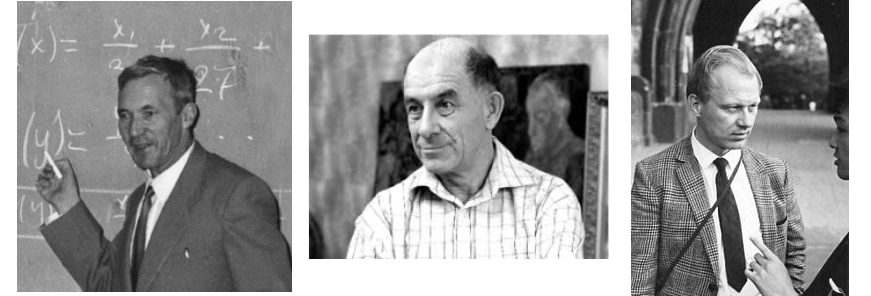
\includegraphics[scale=0.2]{K-A-M.png}}
\caption{Kolmogorov--Arnold--Moser}
\end{figure}


\vspace{-8cm}
\end{frame}

\subsection[Relevancia]{Relevancia}


\begin{frame}
{\structure{\Large ?`Porqué la relevancia?}}
\vspace{-3cm}

\begin{itemize}
\pause
\item Porque resolvería una paradoja de H. Poincaré (del siglo XIX) sobre movimiento planetario y su estabilidad.
\pause
\item Porque ``invalidaría'' la hipótesis ergódica de L. Boltzmann que se encuentra en los fundamentos de la mecánica estadística.
\end{itemize}
\medskip
\pause
\begin{figure}[b]
\only<4>{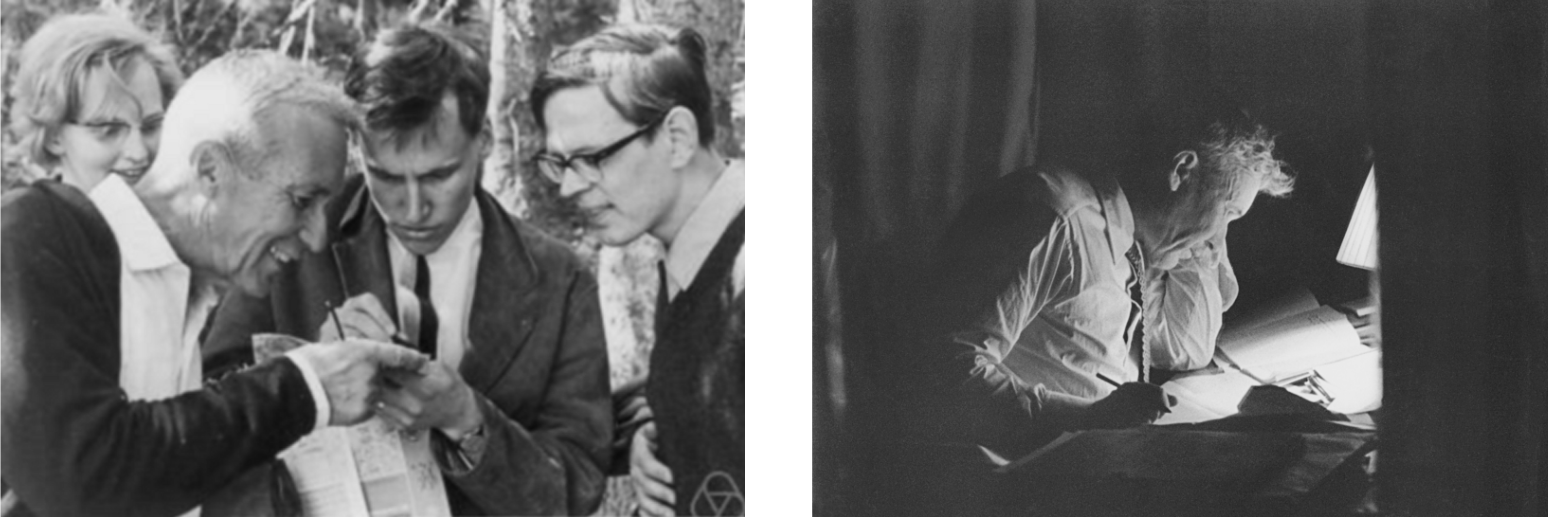
\includegraphics[scale=0.2]{Kol_1-2.png}}
\end{figure}

\vspace{-4cm}
\end{frame}

\subsection[Origen]{Origen}

\begin{frame}
{\structure{\Large Origen}}
\vspace{-0.5cm}

\begin{mybox}{La vieja duda de mecánica celestial:}
?`Es el sistema solar estable?\\
?`Continuará eternamente más o menos como lo vemos hoy?\\
?`Podría ser que la interacción planetaria eventualmente conduzca a catástrofes donde 
ciertos planetas escapen del Sol o colisionen con él?
\end{mybox}
\pause

\begin{figure}[b]
\only<2>{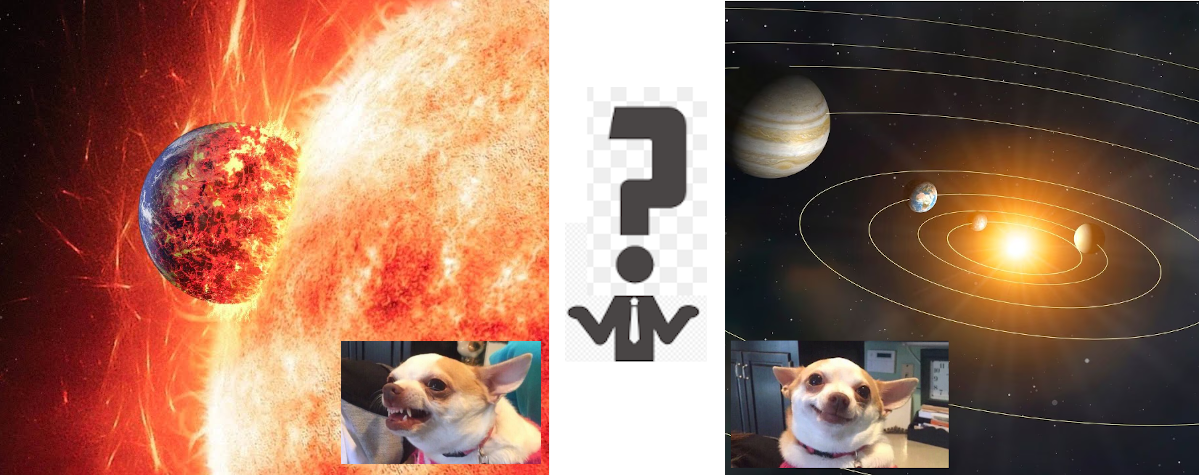
\includegraphics[scale=0.25]{meme.png}}
\end{figure}

\vspace{0cm}
\end{frame}

\section[Conceptos]{Conceptos}

\subsection[Ecuaciones de Newton]{Ecuaciones de Newton}

\begin{frame}{Ecuaciones de Newton}

Un sistema de $n$ masas $m_{0}, \ldots , m_{n}$ con posiciones $x_{0}, \ldots , x_{n}$ 
satisface las leyes de Newton
\be
	m_{i} x_{i}^{\prime \prime} = \sum_{j=0}^{n}  G\, m_{i}m_{j} \frac{x_{j}-x_{i}}{|x_{j}-x_{i}|^{3}},
	\qquad G \approx 6.662 \times 10^{-11} \frac{m^{3}}{kg\, s^{2}} \nonumber
\ee
uno puede simplificar
\bea 
	x_{0}^{\prime \prime} &=& \sum_{j=0}^{n}  G\, m_{j} \frac{x_{j}-x_{0}}{|x_{j}-x_{0}|^{3}} \nonumber \\
	x_{i}^{\prime \prime} &=&  G\, m_{0} \frac{x_{0}-x_{i}}{|x_{0}-x_{i}|^{3}} + \sum_{j=1,j\neq i}^{n}  G\, m_{j} \frac{x_{j}-x_{i}}{|x_{j}-x_{i}|^{3}} \nonumber
\eea

\end{frame}

\begin{frame}{Ecuaciones de Newton}
\vspace{-1cm}

!`Pero! $m_{0}$ es la masa del Sol, luego $m_{0} \gg m_{i}$ y podemos simplificar,
\be 
	x_{0}^{\prime \prime} = 0, \qquad \qquad x_{i}^{\prime \prime} =  G\, m_{0} \frac{x_{0}-x_{i}}{|x_{0}-x_{i}|^{3}}, \nonumber 
\ee
finalmente podemos adoptar un punto de vista heliocéntrico eligiendo $x_{0}=0$, con lo que las ecuaciones de los otros cuerpos se desacoplan
\be 
	x_{i}^{\prime \prime} =  -G\, m_{0} \frac{x_{i}}{|x_{i}|^{3}}.
	\nonumber
\ee

El sistema solar con planetas de ``masa cero'' cumple exactamente con las leyes de Kepler.
En particular este sistema es estable.

\end{frame}

\subsection[Números irracionales]{Números irracionales}

\begin{frame}{Números irracionales}
\vspace{0cm}

\begin{mybluebox}{}
Un concepto central del teorema KAM es la noción de ``suficientemente irracional''.
\end{mybluebox}

Se dice que un número $\theta$ es irracional si $$\left|\theta - \frac{p}{q} \right| \neq 0$$ para todo par de enteros $p, q$.
Pero todo número irracional puede ser aproximado por números racionales,
\be 
	\left|\theta - \frac{p}{q} \right| < \epsilon . \nonumber
\ee

\vspace{0.5cm}

\begin{mybox}{?`Cómo determinar si es una buena o mala aproximación?}
El criterio es la tasa de crecimiento de los denominadores mínimos para aproximaciones más y mas finas lo que determinará una buena o mala aproximación por racionales.
\end{mybox}
\end{frame}

\begin{frame}{Números irracionales}
\vspace{-1cm}

{\bf Ejemplos de aproximación de $\pi$.}
\bigskip

Malas aproximaciones:\\
\be 
	\left|\pi - \frac{314}{100} \right| < \frac{3}{1000}, 
	\qquad \qquad 
	\left|\pi - \frac{314159}{100\, 000} \right| < \frac{3}{1000\, 000}
	\nonumber
\ee
\vspace{0.5cm}

Buenas aproximaciones:\\
\be 
	\left|\pi - \frac{22}{7} \right| < \frac{2}{100}
	\qquad \qquad
	\left|\pi - \frac{355}{113} \right| < \frac{3}{10\, 000\, 000}
	\nonumber
\ee

\end{frame}

\begin{frame}{Números irracionales}
\vspace{-0.5cm}

{\bf Aportacion de Liouville a la Teoría de números.}
\vspace{1cm}

Si $\theta$ es un número algebraico de grado $d$, es decir, que cumple con la ecuación
\be 
	a_{{}_{d}}\theta^{d} + a_{{}_{d-1}}\theta^{d-1}+\cdots + a_{{}_{0}} = 0
	 \nonumber
\ee
con $a_{i}$ enteros, entonces existe una constante $C > 0$ tal que, para todo par de enteros coprimos $p, q$, se tiene
\be 
	\left| \theta - \frac{p}{q} \right| > \frac{C}{q^{d}}.
	\nonumber
\ee
Esto implica que $\theta$ solo puede ser aproximado con racionales con denominadores ``grandes''.\medskip

De aquí se descubrió el primer número trascendente $\sum_{n=0}^{\infty}10^{-n!}$. También $\pi$ y $e$ son trascendentales.

\end{frame}

\begin{frame}{Números irracionales}
\vspace{-0.5cm}

\begin{mygreenbox}{En una formulación más moderna:}
Se dice que un número $\theta$ es {\it suficientemente irracional} si para todo par de números enteros coprimos $p, q$ existe una constante $\gamma_{r}$ tal que
\be 
	\left| q\,\theta - p \right| \geq \frac{\gamma_{r}}{q^{r}} \nonumber
\ee
para un entero $r>1$ arbitrario.
\end{mygreenbox}

Por otro lado, el conjunto de números reales que satisfacen 
\be 
	\left| q\,\theta - p \right| > \frac{\gamma}{q} \nonumber
\ee
es decir $r=1$, es de medida cero. 

\end{frame}

\begin{frame}{Irracionalidad de vectores}
\vspace{-1cm}

Considérese el vector $\left(\omega_{1}, \ldots , \omega_{n} \right)$ formado por las frecuencias $\omega_{i}=\frac{1}{P_{i}}$ donde $P_{i}$ es el periodo del $i$-ésimo planeta de un sistema planetario.
\bigskip

El análogo de la condición de ``irracionalidad suficiente''  para vectores de longitud $n$ es 
\be 
	\left|k_{1}\omega_{1} + \cdots + k_{n}\omega_{n} \right|
	\geq \frac{\gamma}{(k_{1}^{2} + \cdots + k_{n}^{2})^{n/2}}
	\nonumber
\ee
para todo vector $(k_{1}, \ldots ,k_{n})$ de coeficientes enteros y alguna constante $\gamma > 0$.
\medskip

El subconjunto de vectores $(\omega_{1}, \ldots , \omega_{n}) \in \mathbb{R}^{n}$ que satisfacen la condición anterior, son de medida completa, es decir, que su complemento tiene medida cero.


\end{frame}

\section[Teorema KAM]{Teorema KAM}

\subsection[KAM limitado]{KAM limitado}

\begin{frame}{KAM para sistemas solares}
\vspace{-1.0cm}

\begin{itemize}
\item El movimiento planetario bajo la hipótesis de planetas de masa cero describe trayectorias elípticas, que son topológicamente círculos.
\item Pensemos en el círculo como el espacio cociente $\mathbb{R}/\mathbb{Z}$, donde se identifican los números que difieren por un entero, esto es: Dados $u, v \in \mathbb{R}$ decimos que están relacionados módulo $\mathbb{Z}$ si $u-v \in \mathbb{Z}$.
\item Identificamos un toro $n$-dimensional como el espacio $\left(\mathbb{R}/\mathbb{Z}\right)^{n}$. Este espacio considera las trayectorias de $n$ planetas.
\item Las trayectorias sobre el toro están parametrizadas por el tiempo $t \mapsto \vec{a} + t \vec{\omega}$, donde $\vec{a} = (a_{1}, \ldots, a_{n})$ y $\vec{\omega} = (\omega_{1},\ldots , \omega_{n})$, de modo que 
\be 
	v(t) = (a_{1} + t \omega_{1}, \ldots, a_{n} + t \omega_{n})
	\nonumber
\ee
este movimiento se conoce como {\it flujo lineal sobre} $\left(\mathbb{R}/\mathbb{Z}\right)^{n}$ {\it en la dirección} $\vec{\omega}$.
\item Las trayectorias sobre el toro serán densas sí y solo sí $\vec{\omega}$ es irracional. Si todas las trayectorias son múltiplos de una frecuencia común, entonces la trayectoria es un círculo embebido en el toro.
\end{itemize}

\end{frame}

\begin{frame}{KAM para sistemas solares}
\vspace{-0.0cm}

\begin{figure}[h]
\centering
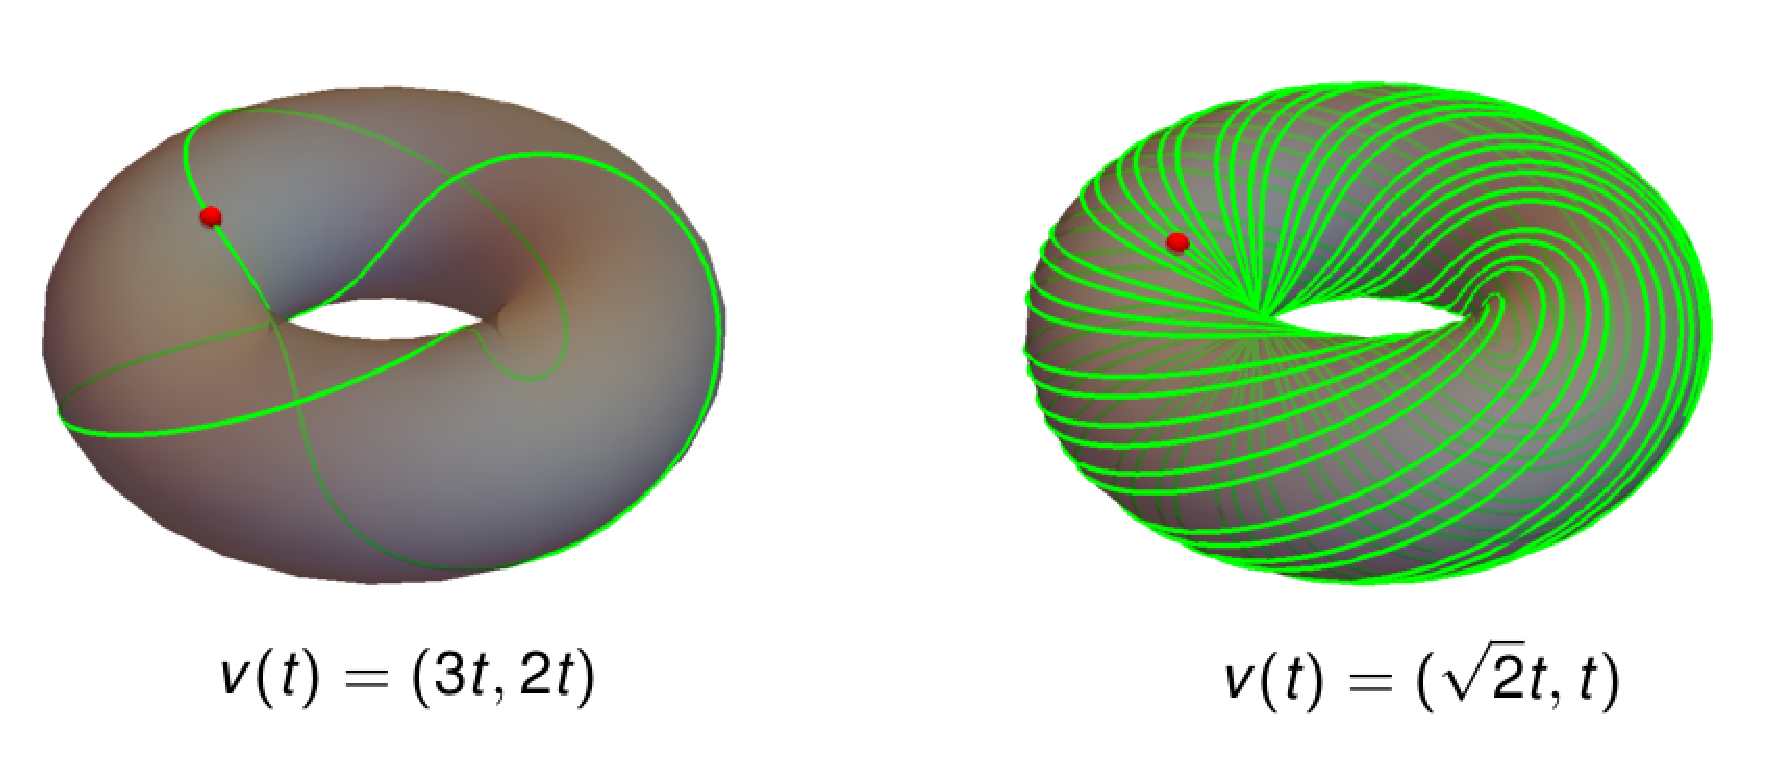
\includegraphics[scale=0.35]{toros.eps}
\end{figure}

\end{frame}

\begin{frame}{KAM para sistemas solares}
\vspace{-0.0cm}

\begin{figure}[h]
\centering
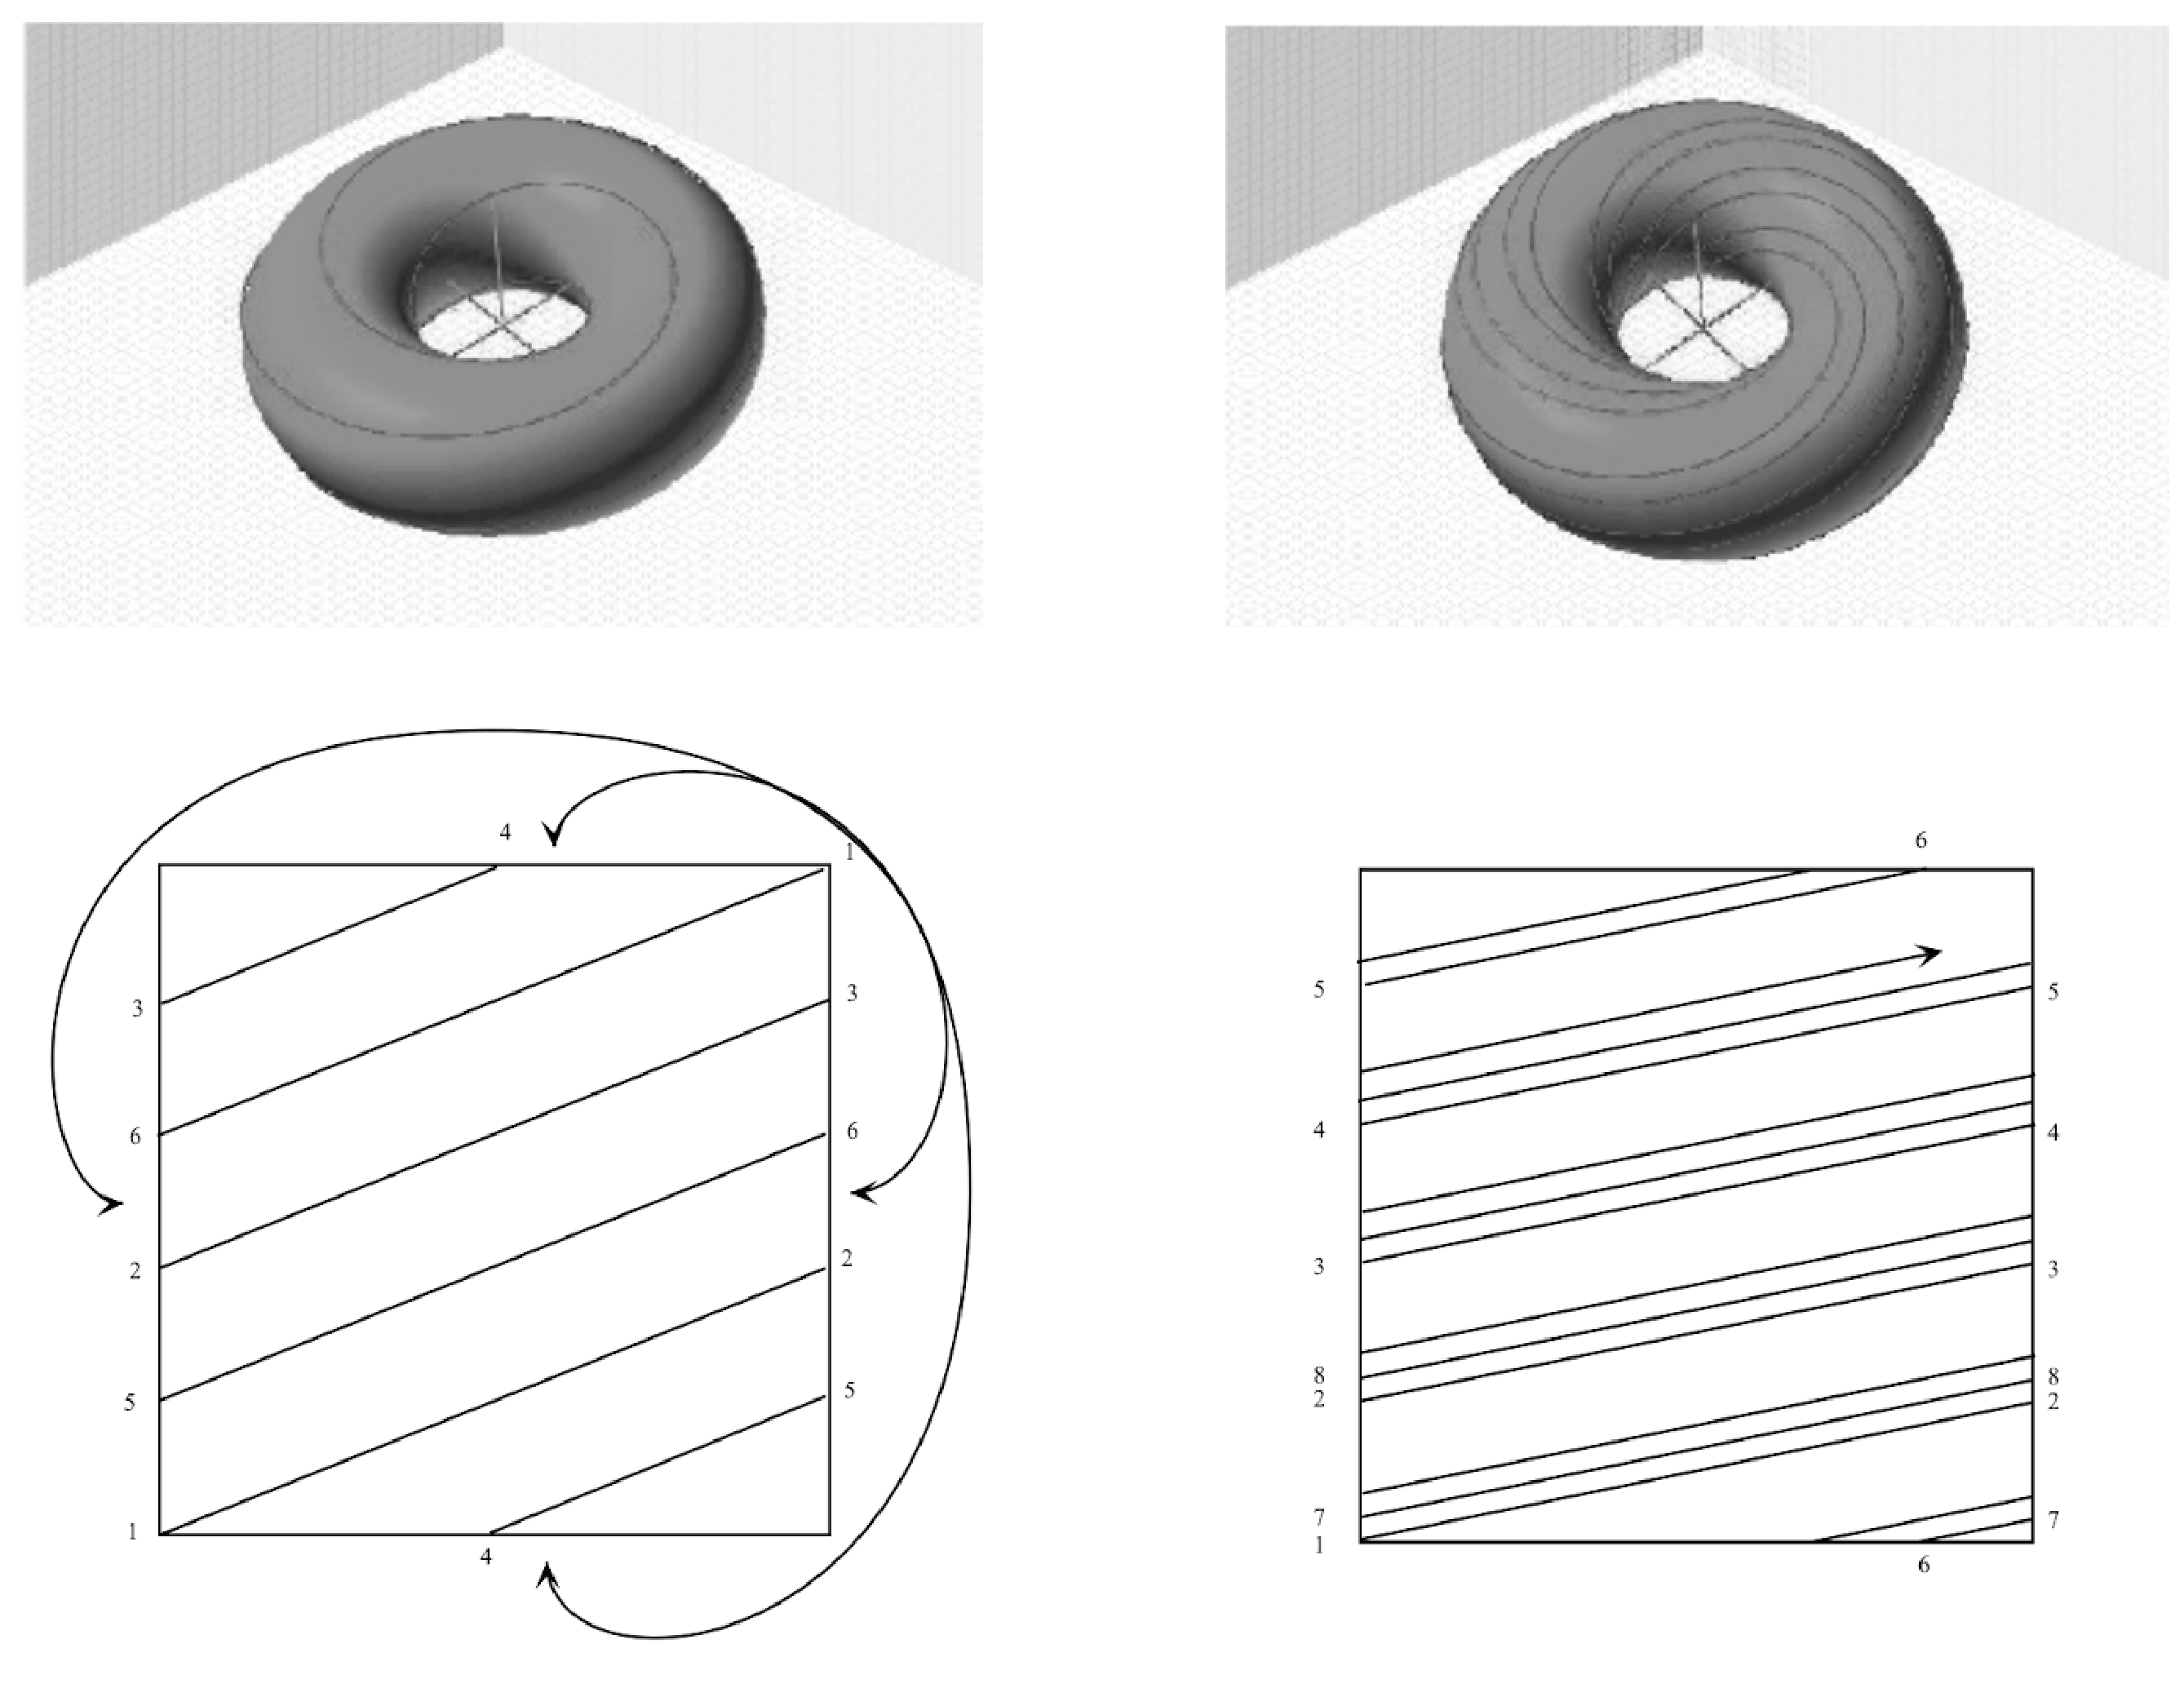
\includegraphics[scale=0.2]{comb.eps}
\end{figure}

\end{frame}

\begin{frame}{KAM para sistemas solares}
\vspace{-0.0cm}

\begin{mygreenbox}{}
\centering
Decimos que un movimiento $v(t)$ de un sistema perturbado\\[5pt] es ``el mismo'' que el de un movimiento denso no perturbado\\[5pt] $v_{0}(t)$ sobre el toro $T_{0}$, cuando $v(t)$ es denso sobre un toro $T$\\[5pt] \hspace{-0.3cm} y $v(t)$ llena $T$ en la misma forma combinatoria que $v_{0}(t)$ lo\\[5pt] \hspace{-4.7cm} hace sobre $T_{0}$, esto es: \\[5pt]
Existe un homeomorfismo $\Phi:T \rightarrow T_{0}$, tal que, $\Phi(v(t)) = v_{0}(t)$.
\end{mygreenbox}

\footnote{Un homeomorfismo es una función de un espacio topológico a otro\\ que cumple con ser biyectiva continua y cuya inversa es continua.} 
\end{frame}

\begin{frame}{KAM para sistemas solares}
\vspace{-0.0cm}

\begin{mybox}{Teorema KAM para sistemas solares}
Sea $v_{0}(t)$ un movimiento de sistemas de masa cero, que posee un vector de\\[5pt] frecuencias ``suficientemente irracional'', de modo que $v_{0}$ es denso sobre el toro $T_{0}$.\\[5pt]
Entonces, existe $\epsilon > 0$ tal que, si los planetas tienen masas $m_{i} < \epsilon$,\\[5pt] existe una trayectoria $v(t)$ del sistema perturbado, denso sobre un toro $T$,\\[5pt] y un homeomorfismo $\Phi: T \rightarrow T_{0}$, tal que, $\Phi(v(t))=v_{0}(t)$.
\vspace{0.5cm}

Además, el conjunto de trayectorias de este tipo es un conjunto de medida positiva en el conjunto de todas las trayectorias, y la probabilidad de estar en una de tales trayectorias tiende a 1 cuando $\epsilon$ tiende a 0.
\end{mybox}

\end{frame}

\subsection[Digresiones]{Digresiones}

\begin{frame}{Digresiones}

\begin{mybluebox}{}
El teorema KAM establece que si un sistema mecánico totalmente integrable admite\\[2pt] trayectorias suficientemente irracionales, entonces cada perturbación del sistema\\[2pt] suficientemente pequeña también admite ``el mismo movimiento''. 
\end{mybluebox}
\bigskip

\begin{mybluebox}{?`Nuestro sistema solar está en una de esas trayectorias estables descritas por el teorema KAM?}
\textbf{No}, porque las orbitas de Jupiter y Saturno están en una razón de $5:2$, \\[2pt] entonces no se cumple la hipótesis. !`Pero! Refinamientos del teorema KAM \\[2pt] garantizan que existen también zonas de movimientos estables aún cuando hay \\[2pt]proporciones racionales, en ``zonas de segundo orden''.
\end{mybluebox}
\end{frame}

\begin{frame}{Digresiones}

\begin{mybluebox}{}
Desde un punto de vista sociológico, un sistema, en general, requiere de leyes que\\[2pt] definan aquello que puede hacer, pues el estado normal de la anarquí es el caos.\\[2pt] Desde este punto de vista deberíamos esperar que en ausencia de leyes de conservación,\\[2pt] los movimientos típicos del sistema se pierdan. Sin embargo, el teorema KAM niega\\[2pt] esto diciendo que cuando las leyes son relajadas un poco, la mayoría de movimientos\\[2pt] ``prácticamente'' se quedan donde estaban.
\end{mybluebox}

\begin{mybluebox}{?`Por qué pensar que esto es verdad?}
Si imaginamos que de hecho lo que ocurre fuera lo contrario, y tan pronto como las leyes\\[2pt] de conservación se perdieran las trayectorias se fueran a todos lados, la existencia del\\[2pt] sistema solar mismo sería improbable, pues el estado genérico de todo sistema mecánico\\[2pt] sería el caos.
\end{mybluebox}

\end{frame}

\subsection[Otro repaso]{Otro repaso}

\begin{frame}{Otro repaso de conceptos y definiciones}

\begin{itemize}
\item[$\hookrightarrow$] \textbf{Espacio de configuraciones $\mathbf{M}$} de un sistema de $n$ grados de libertad es aquel en el que ``habitan'' todos los posibles valores de las coordenadas que describen al estado del mismo.\\[10pt]
\item[$\hookrightarrow$] $\mathbf{M}$ siempre puede ser dotado de una estructura de variedad diferenciable $n$-dimensional.\\[10pt]
\item[$\hookrightarrow$] \textbf{Espacio tangente $\mathbf{T_{x}M}$} a un punto $x \in \mathbf{M}$ es el conjunto de todos los vectores tangentes a $x$.\\[10pt]
\item[$\hookrightarrow$] \textbf{Fibrado tangente $\mathbf{TM}$} es el conjunto de los espacios tangentes $\mathbf{T_{x}M}$, en todos los puntos $x \in M$. Este espacio es de dimensión $2n$.\\[10pt]
\item[$\hookrightarrow$] \textbf{Fibrado cotangente $\mathbf{T^{\ast}M}$} es el dual algebraico del espacio tangente. También es conocido como espacio fásico, es $2n$-dimensional y su utilidad radica en su {\it estructura simpléctica}.
\end{itemize}

\end{frame}

\begin{frame}{Otro repaso de conceptos y definiciones}

\begin{itemize}
\item[$\hookrightarrow$] {\bf Una $2$-forma simpléctica} sobre el espacio vectorial $V$ es una función $\sigma : V \times V \rightarrow \mathbb{R}$ tal que
\begin{itemize}
\item $\sigma$ es bilineal
\item $\sigma$ es antisimétrica.
\item $\sigma$ es no-degenerada.\\[10pt]
\end{itemize}
\item[$\hookrightarrow$] {\bf Un espacio simpléctico} es la dupla $(V,\sigma)$.\\[10pt]
\item[$\hookrightarrow$] {\bf La 2-forma hamiltoniana} es la forma simpléctica $\sigma : \mathbf{T^{\ast}M} \times \mathbf{T^{\ast}M} \rightarrow \mathbb{R}$, definida como $\sigma(v,w) = \< v,\Omega w \>$, donde $v, w \in \mathbf{T^{\ast}M}$, $\< \cdot , \cdot \>$ es el producto interior y $\Omega$ es la métrica simpléctica, cuya forma matricial es
\be 
	\Omega = \begin{pmatrix}
	\mathbf{0}_{n} & \mathbf{1}_{n} \\
	-\mathbf{1}_{n} & \mathbf{0}_{n}
	\end{pmatrix} \nonumber 
\ee
\item[$\hookrightarrow$] {\bf El paréntesis de Poisson} es la 2-forma hamiltoniana,
\be 
	\{ f, g \} =\sigma(\nabla f, \nabla g) = \< \nabla f, \Omega \nabla g \>,
	\qquad f,g : \mathbf{T^{\ast}M} \rightarrow \mathbb{R} \nonumber
\ee
\item[$\hookrightarrow$] {\bf Gradiente simpléctico}, en este contexto, es la forma en que se conoce a $\nabla_{\Omega} g = \Omega \nabla g$.
\item[$\hookrightarrow$] {\bf Una transformación canónica $\mathbf{S}$}, en forma matricial, es aquella que deja invariante la métrica simpléctica, esto es, $$\mathbf{S}\Omega\mathbf{S}^{\dagger} = \Omega .$$
\end{itemize}
\end{frame}

\begin{frame}{Otro repaso de conceptos y definiciones}

\begin{mybox}{Teorema para sistemas integrables}
Consideremos un sistema con $n$ grados de libertad, del cual se conocen $n$ integrales primeras $\{f_{1}, \ldots, f_{n}\}$. Definimos:
\be 
	\mathbf{T^{\ast}M_{f}} = \left\lbrace \eta \in \mathbf{T^{\ast}M}\, | \, f_{i}(\eta) = f_{i0}, \ i=1, \ldots, n \right\rbrace \nonumber
\ee
donde $f_{i0}$ son constantes. Supongamos que:
\begin{itemize}
\item El conjunto de $\{f_{1}, \ldots, f_{n}\}$ son independientes en cada punto de $\mathbf{T^{\ast}M_{f}}$ en el sentido de que sus gradientes son linealmente independientes.
\item $\{f_{i}, f_{j} \}=0$ para todo $i,j$, es decir, están en involución.
\end{itemize}
Entonces, $\mathbf{T^{\ast}M_{f}}$ es una $n$-subvariedad del espacio $\mathbf{T^{\ast}M}$ 
y el movimiento se queda confinado por completo en $\mathbf{T^{\ast}M_{f}}$, siendo $H = f_{j}$ para alguna $j$. Además si $\mathbf{T^{\ast}M_{f}}$ es compacta y conexa, es difeomorfa al toro $T^{n}$.
\end{mybox}

Si nuestro sistema es integrable, el teorema anterior garantiza que existe una transformada canónica (variables de ángulo-acción) que verifica que el hamiltoniano solo depende del momento momento (acción).
\end{frame}


\subsection[KAM general]{KAM general}

\begin{frame}{Teorema KAM}

Sea $(\mathbf{T^{\ast}M},\sigma)$ una variedad simpléctica asociada a un sistema totalmente integrable con $n$ grados de libertad, tal que, $\mathbf{T^{\ast}M} = T^{n} \times \mathbb{R}^{n}$, con variables $q\in T^{n}$ y $p \in \mathbb{R}^{n}$ y forma simpléctica $\sigma = \<\nabla f, \Omega \nabla g \>$. \\[10pt]

La ecuación diferencial hamiltoniana se expresa en la forma $$\dot{x} = \left(\nabla_{{}_{\Omega}}H\right)(x)$$ donde $x^{T} = (q,p)$. Denotaremos por $\phi_{H}^{t}$ el flujo del campo vectorial $\nabla_{{}_{\Omega}}H$.\\[10pt]

Debido a que el sistema es integrable, es posible expresar el hamiltoniano $H(p)$ como función únicamente de $p$. La ecuación diferencial hamiltoniana conduce a la solución
\be 
	p(t) = p_{0}, \qquad  \qquad
	q(t) = q_{0} + t \frac{\partial H}{\partial p}(p_{0}) = q_{0} + t \omega(p_{0}) 
	\nonumber
\ee 
cada coordenada $p_{1}, \ldots, p_{n}$ se conserva y la trayectoria está en el toro $T^{n} \times p_{0}$.

\end{frame}

\begin{frame}{Teorema KAM}

Definimos 
\be 
	P_{\delta} = \lbrace p \in \mathbb{C}^{n} \, | \, |p| \leq \delta \rbrace
	\qquad 
	\qquad 
	Q_{\delta} = \lbrace q \in \mathbb{C}^{n}/\mathbb{Z}^{n} \, | \, |Im(q)| \leq \delta \rbrace \nonumber
\ee
\vspace{0.1cm}
\be 
	A_{\delta} 
	= Q_{\delta} \times B_{\delta} 
	= \lbrace (q,p) \in \mathbb{C}^{n}/\mathbb{Z}^{n} \times \mathbb{C}^{n} \, | \,  |p| \leq \delta, \, |Im(q)| \leq \delta \rbrace \nonumber
\ee
y denotamos por $\mathcal{P}_{\delta}$, $\mathcal{Q}_{\delta}$, $\mathcal{A}_{\delta}$ a las álgebras de Banach de funciones continuas sobre estos conjuntos, con la norma del supremos $\parallel f \parallel_{\delta}$.

\vspace{1cm}

Un álgebra de Banach $\mathcal{A}$ es un álgebra asociativa sobre los reales o los complejos que además es un espacio normado y completo bajo la métrica inducida por una norma que satisface 
\be 
	\parallel x \cdot y \parallel \, \leq \, \parallel x \parallel \ \parallel y \parallel
	\nonumber
\ee
para todo $x,y \in \mathcal{A}$.

\end{frame}

\begin{frame}{Teorema KAM}

\begin{mybox}{Teorema KAM}

Sean $\delta, \gamma > 0$ dos números y sea $h(q,p) = h_{0}(p) + h_{1}(q,p)$ un hamiltoniano con $h_{0} \in \mathcal{P}_{\delta}$, $h_{1} \in \mathcal{A}_{\delta}$ 
y $\parallel h_{0} \parallel_{\delta} \leq 1$. Escribimos la expansion
\be 
	h_{0}(p) = a + \omega \cdot p + \onehalf p \cdot C p + o(|p|^{2}),
	\nonumber 
\ee
la expansión de orden $2$ de $h_{0}$, con $omega$ suficientemente irracional y $C$ una matriz simétrica e invertible. Entonces para todo $\delta_{\ast} <  \delta$ existe $\epsilon > 0$, dependiente de $C$ y de $\gamma$ pero no del termino $o(|p|^{2})$, tal que
cuando $\parallel h_{1} \parallel_{\delta} \leq \epsilon$, existe un mapa simpléctico $\Phi: A_{\delta_{\ast}} \rightarrow A_{\delta}$ tal que, estableciendo $(q,p) = \Phi(q^{\prime},p^{\prime})$ y $H = h \circ \Phi$, tenemos
\be 
	H(q^{\prime},p^{\prime}) = A + \omega \cdot p^{\prime} + R(q^{\prime},p^{\prime})
	\nonumber
\ee 
donde $R(q^{\prime},p^{\prime}) \in O(|p^{\prime}|^{2})$.

\end{mybox}

\end{frame}

\begin{frame}{Interpretación del KAM}

\begin{mygreenbox}{KAM}

Si un sistema es hamiltoniano, integrable y no degenerado, cuando se le introduce una perturbación de la misma forma, con amplitud $\varepsilon$,
\be 
	H(q,p) = H_{0}(p) + \varepsilon H_{1}(q,p) \nonumber
\ee
la probabilidad de escoger unas condiciones iniciales correspondientes a un toro que` no haya sido destruido por la perturbación tiende a $1$ cuando $\varepsilon$ tiende a $0$. Esos toros están ligeramente deformados por la acción de dicha perurbación, pero existe un límite en que los toros `evientan'', no se pueden deformar a voluntad.

\end{mygreenbox}

\end{frame}

\subsection[Consecuencias en el péndulo forzado]{Consecuencias en el péndulo forzado}

\begin{frame}{Péndulo forzado}

Ecuación del péndulo forzado:
\be 
	x^{\prime \prime} +\sin x = \varepsilon \cos 2\pi t \nonumber
\ee
simplificada
\be 
	x^{\prime} = y, \qquad \qquad
	y^{\prime} = - \sin x + \varepsilon \cos 2\pi t.
	\nonumber
\ee
\vspace{0.5cm}

\begin{mybox}{Teorema}

Para todo periodo $\alpha > 2\pi$ existe $c$ tal que si $|\varepsilon| < c$, entonces la solución tiene un periodo $\alpha$. El conjunto de esas soluciones tiene medida positiva.  

\end{mybox}

\end{frame}

\begin{frame}{Péndulo forzado}

\begin{figure}[h]
\centering
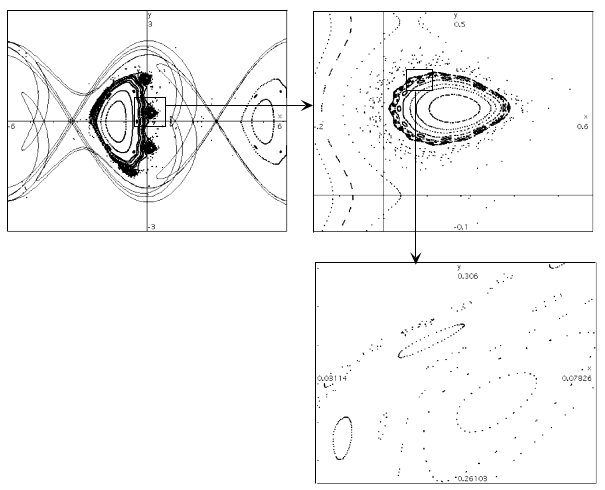
\includegraphics[scale=0.4]{pendulo.png}
\caption{Áreas de orden y caos para $\varepsilon=0.3$.}
\end{figure}

\end{frame}

\end{document}
